
\documentclass{beamer}

\usepackage{graphicx}
\usepackage[light]{FiraSans}
\usepackage[british]{datetime2}
\usepackage{tabularx}
\usetheme{default}
\setbeamertemplate{navigation symbols}{} % No navigation symbols
\definecolor{ntnu}{cmyk}{100,75,0,5}
\setbeamercolor{alerted text}{fg=ntnu}
\setbeamercolor{frame title}{fg=ntnu}
\setbeamercolor{title}{fg=ntnu}
\setbeamercolor{subtitle}{fg=ntnu}
\setbeamercovered{transparent}

%\setbeamertemplate{itemize item}{\color{white}$\bullet$} 
% Include above line to remove bullet indicators

\setbeamertemplate{footline}{
\begin{tabularx}{\textwidth} {
	 >{\raggedright\arraybackslash}X 
  	 >{\centering\arraybackslash}X 
  	 >{\centering\arraybackslash}X 
  	 >{\centering\arraybackslash}X 
  	 >{\centering\arraybackslash}X 
  	 >{\centering\arraybackslash}X}
	
	\raisebox{-0.3cm}
	{
\includegraphics[width=2cm, keepaspectratio]{logo_ntnu_u-slagord.pdf}} &
	\insertshortauthor & 
	\insertshorttitle &
	\insertdate &
	\insertsection &
	$\big|$ \insertframenumber
\end{tabularx}
}

\makeatletter
\makeatother

%----------------------------------------------------------------------------------------
%	TITLE PAGE
%----------------------------------------------------------------------------------------

\title[POL2012]{POL2012: Theories and Models in Political Economy}
\subtitle{The financial crisis, recession and stagnation} % Discussion time!
\date{\today}
\author{Marius Swane Wishman}
\institute{Department of Sociology and Political Science}

\begin{document}

\begin{frame}[plain]
\titlepage 
\centering

\includegraphics[width=5cm]{logo_ntnu_u-slagord.pdf} 
\end{frame}

\section{The global financial crisis}

\begin{frame}{The global financial crisis}
\begin{columns}{}
\column{0.5\textwidth}
\begin{itemize}
    \item Real estate bubble\pause
    \item Home prices up 60\% 2000-2006\pause
    \item Subprime loans\pause
    \item Securitization\pause
    \item Crisis goes global
\end{itemize}{}
\column{0.5\textwidth}
\begin{figure}
    \centering
    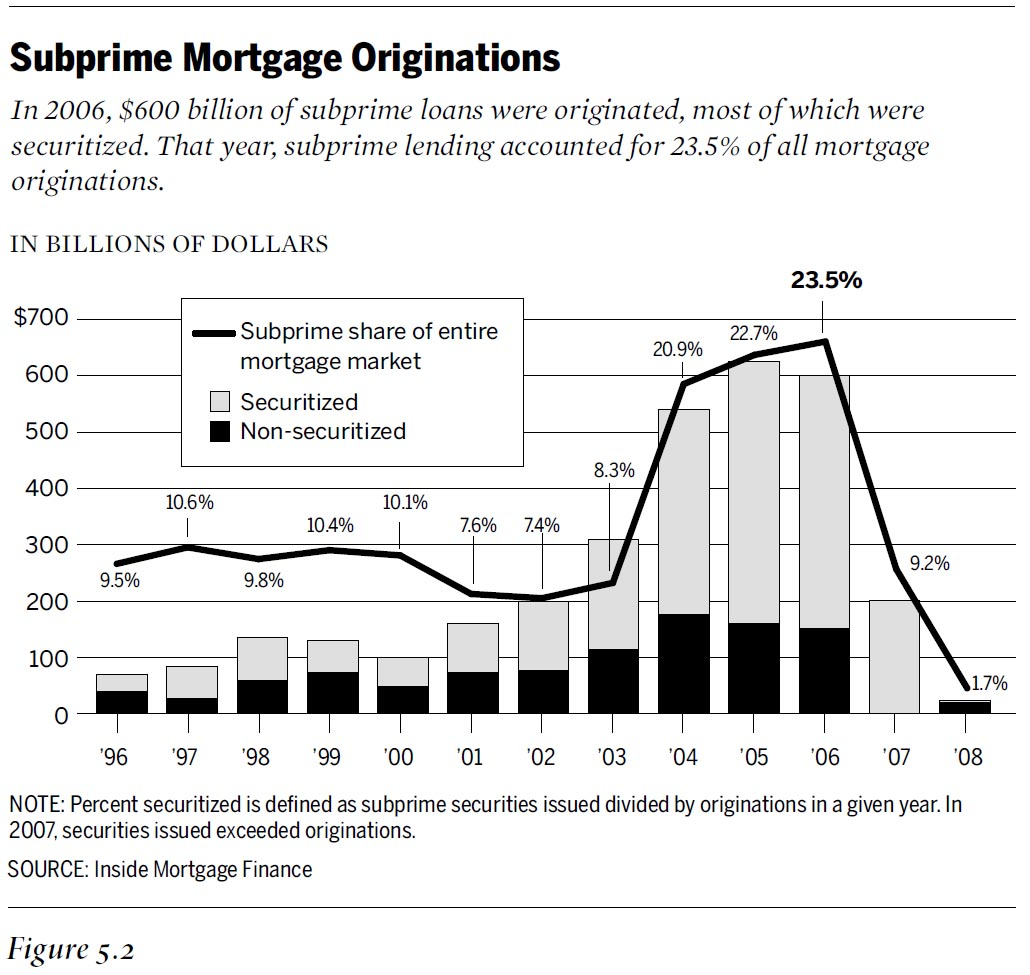
\includegraphics[width=\textwidth]{../img/subprime.jpg}
\end{figure}{}
\end{columns}
\end{frame}{}

\begin{frame}{}
\begin{figure}
    \centering
    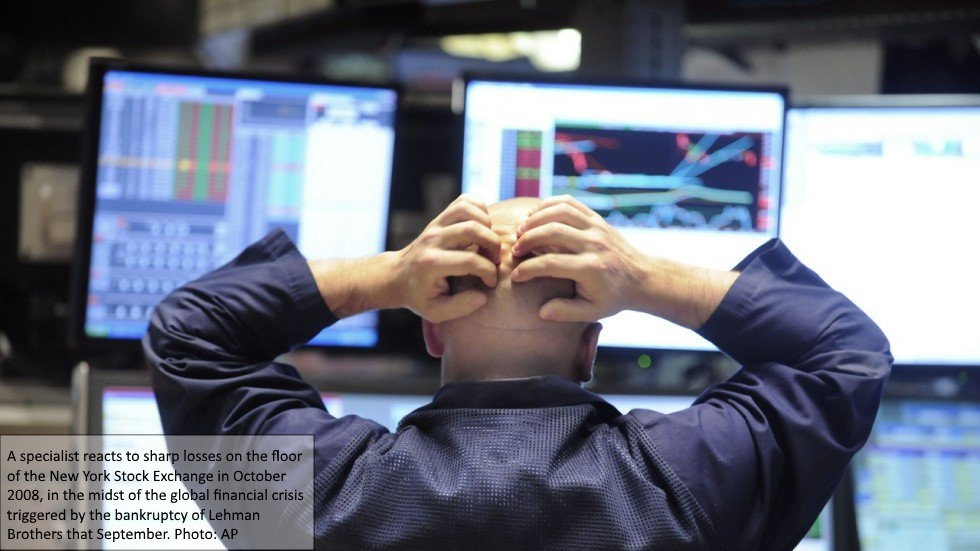
\includegraphics[width=\textwidth]{../img/crash.JPG}
\end{figure}
\end{frame}{}

\section{Discussion}

\begin{frame}{}
\centering
\alert{\Large{But why did it happen?}}
% What do you think?
%---
% What would Marx, Keyens (not really relevant until maaybe the recovery! Unnamed institutionalist instead)  or Friedman say?
% Inevitable consequence of the system. Capitalists seeking profits but the rates of profits are getting ever smaller! This also explains why the crisis became so big.
% Lack of regulation! Investment bank subject to less oversight than regular banks and who polices the police? (insurance)
% Government programs encouraging home ownership, Fed too low interest rates (until sudden increase) + increasing housing prices + other technicalities (market to market accounting). Wesbury (a bit on the extreme).
\end{frame}{}

\section{Response}

\begin{frame}{Response}
\begin{itemize}
    \item \$200 billion injected into the market by the Fed, the ECB and the Bank of England\pause % Keynes!
    \item Expansionary monetary policy $\rightarrow$ low interest-rates\pause
    \item United States continued stimulus in the range of \$800 billion \pause
    \item ECB turned to fiscal discipline\pause
    \begin{itemize}
        \item Sovereign debt
    \end{itemize}{}
\end{itemize}{}
\end{frame}

\begin{frame}{The problem of diversity}
\begin{itemize}
    \item What is appropriate for Germany may not be appropriate for certain other EU countries\pause
    \item And vice-versa\pause
    \item The United States has this problem too!\pause
    \item However, it is easier to get Americans to bail out fellow Americans
\end{itemize}
\end{frame}

\begin{frame}{}
\centering
\alert{\Large{Who do you think fared better?}}
\end{frame}

\begin{frame}{Recovery}
\begin{figure}
    \centering
    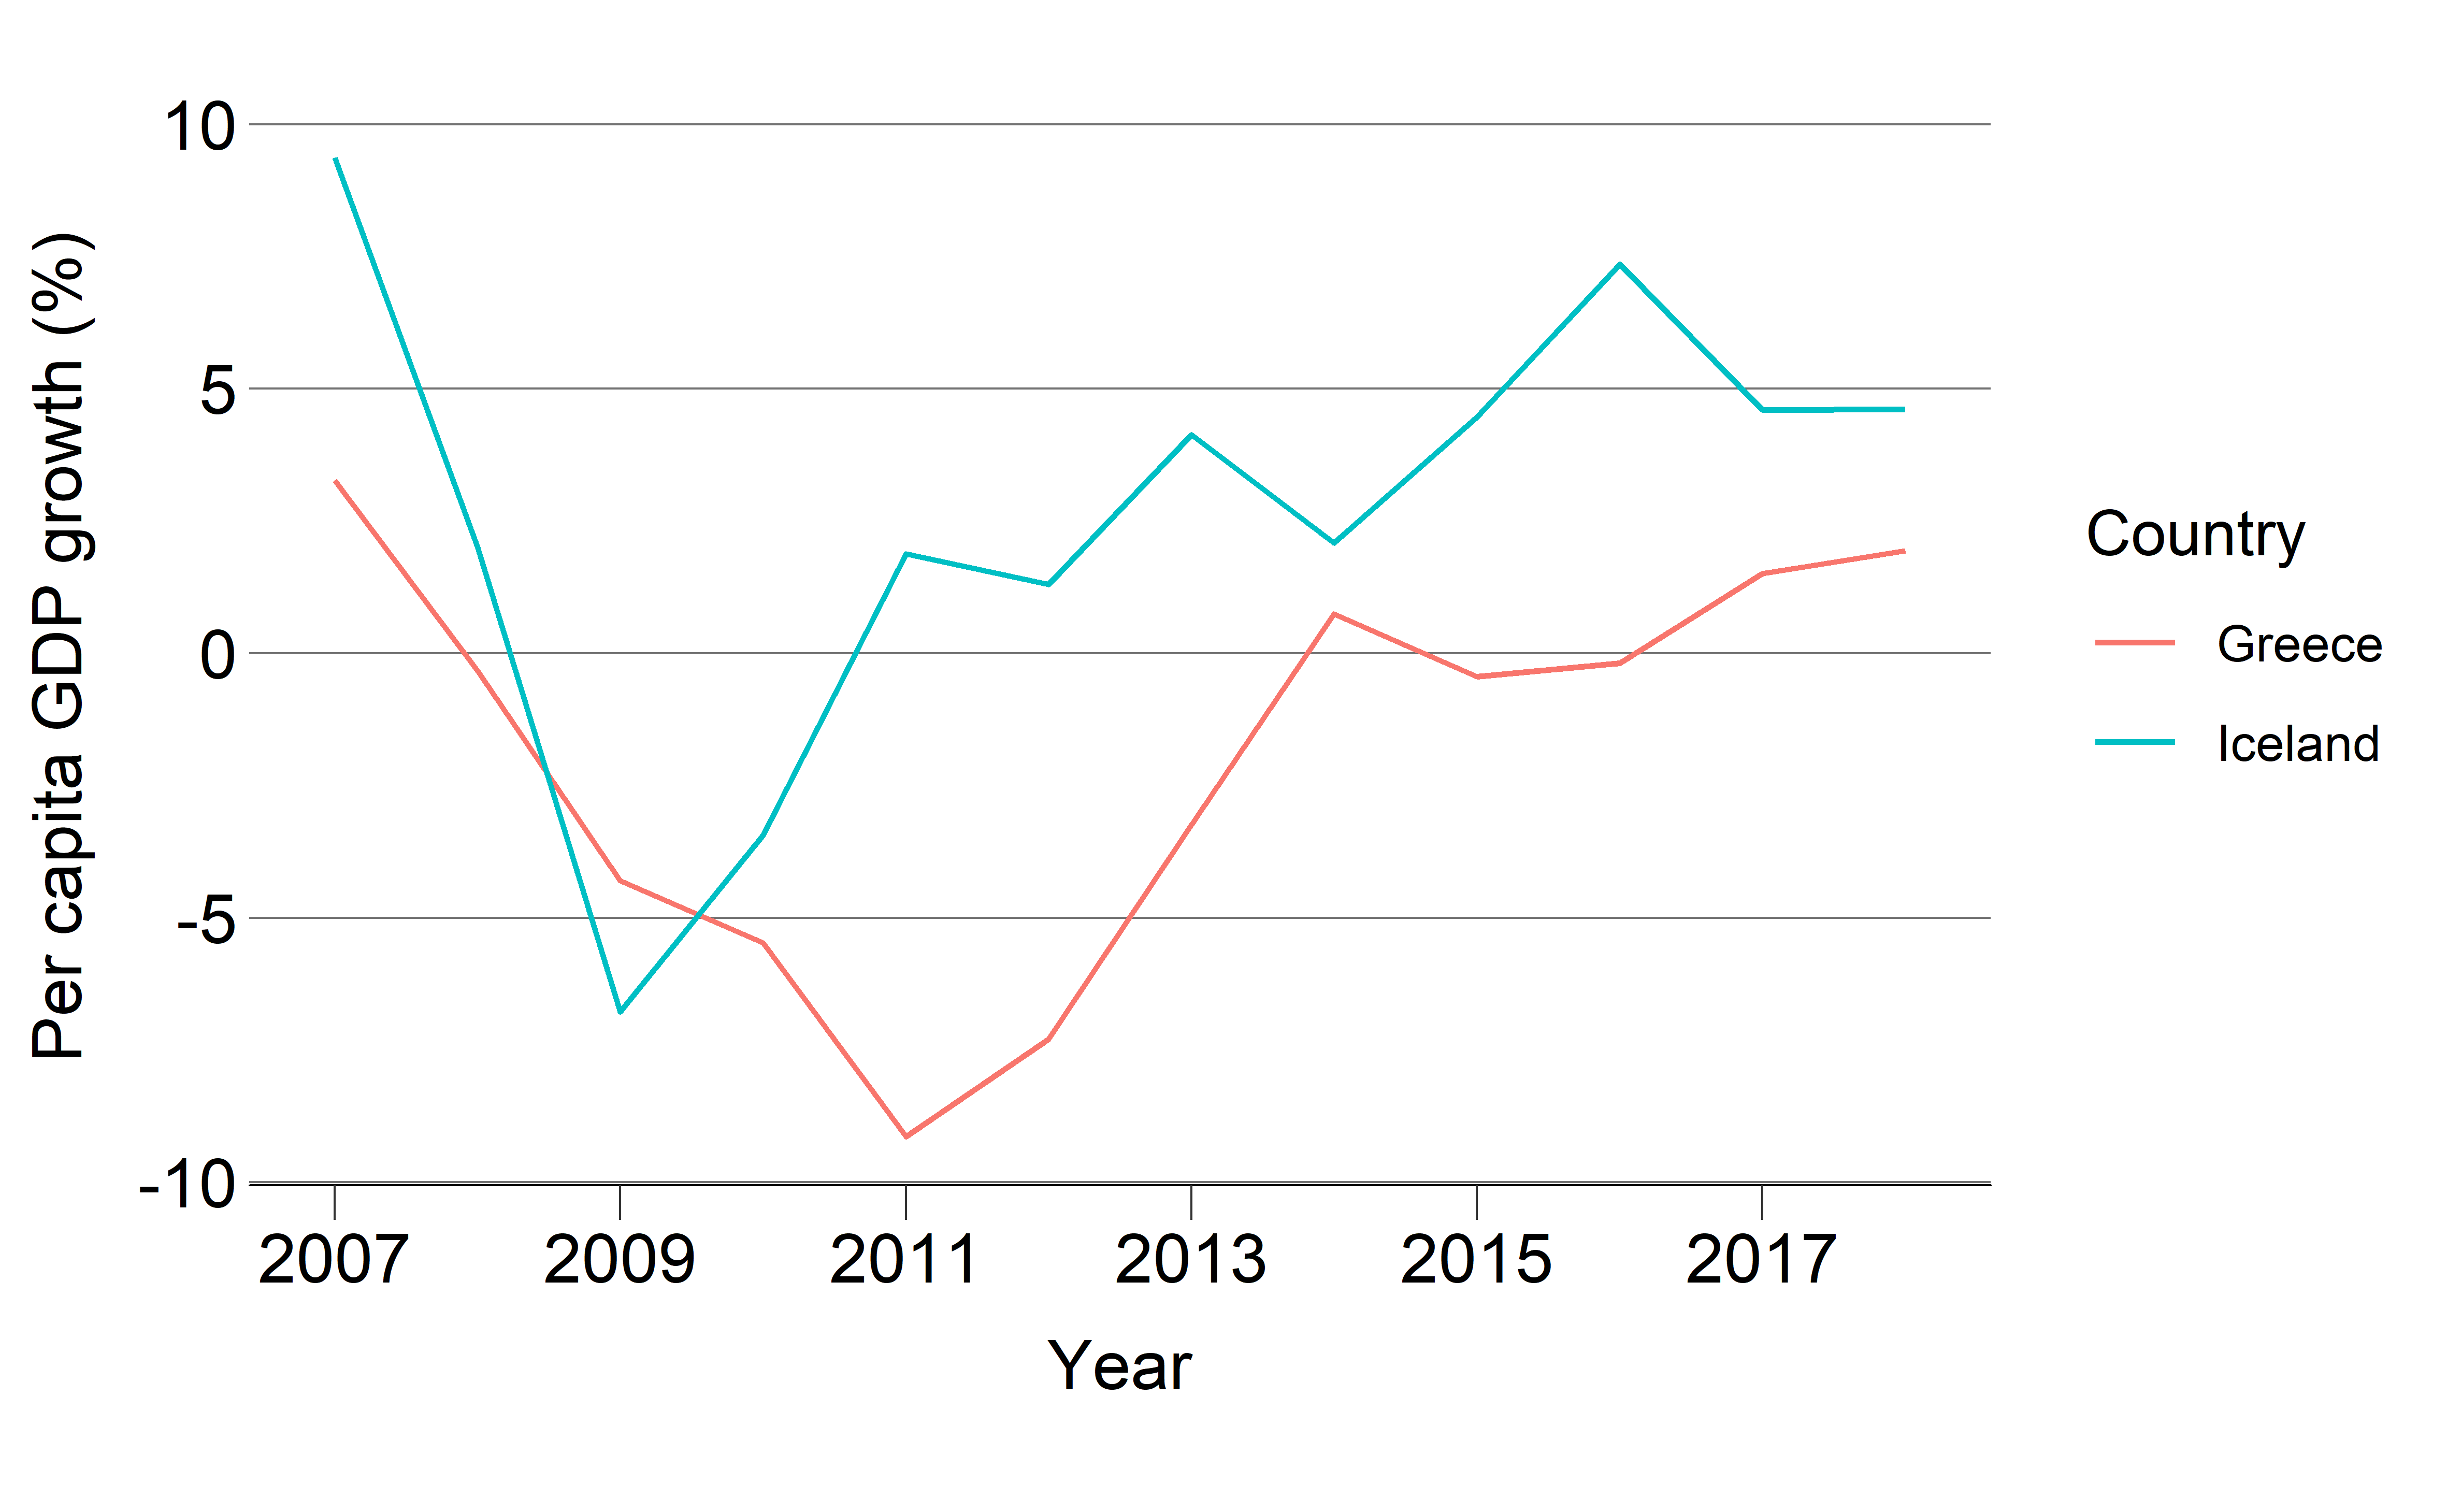
\includegraphics[width=\textwidth]{../img/recovery.png}
\end{figure}{}
\end{frame}{}

\section{Discussion}

\begin{frame}{Lazy Southern Europeans or draconian Germans?}
\begin{figure}
    
\includegraphics[width=0.5\textwidth]{../img/siesta.jpg}
    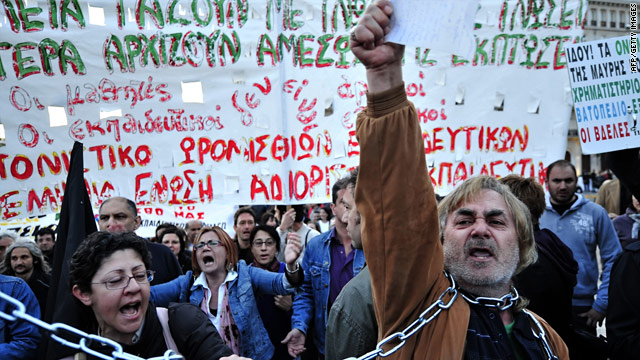
\includegraphics[width=0.5\textwidth]{../img/austerity.jpg}    
\end{figure}{}
\end{frame}{}

\begin{frame}{Some perspectives}
\begin{itemize}
    \item Piketty: ``Germany has never repaid its debts. It has no right to lecture Greece."\pause
    \begin{itemize}
        \item Two ways to repay debt:
        \begin{itemize}
            \item Strict budgetary discipline over 100 years\pause
            \item Inflation, tax on private wealth, debt relief\pause
        \end{itemize}{}
    \end{itemize}{}
    \item Krugman: Eliminating deficits during a crisis is a recipe for depression. Leave the Euro.\pause
    \item Ferguson: Clean slate makes no sense if the problem is structural 
\end{itemize}{}
\end{frame}{}

\begin{frame}{Greeceland}
\begin{figure}
    \centering
    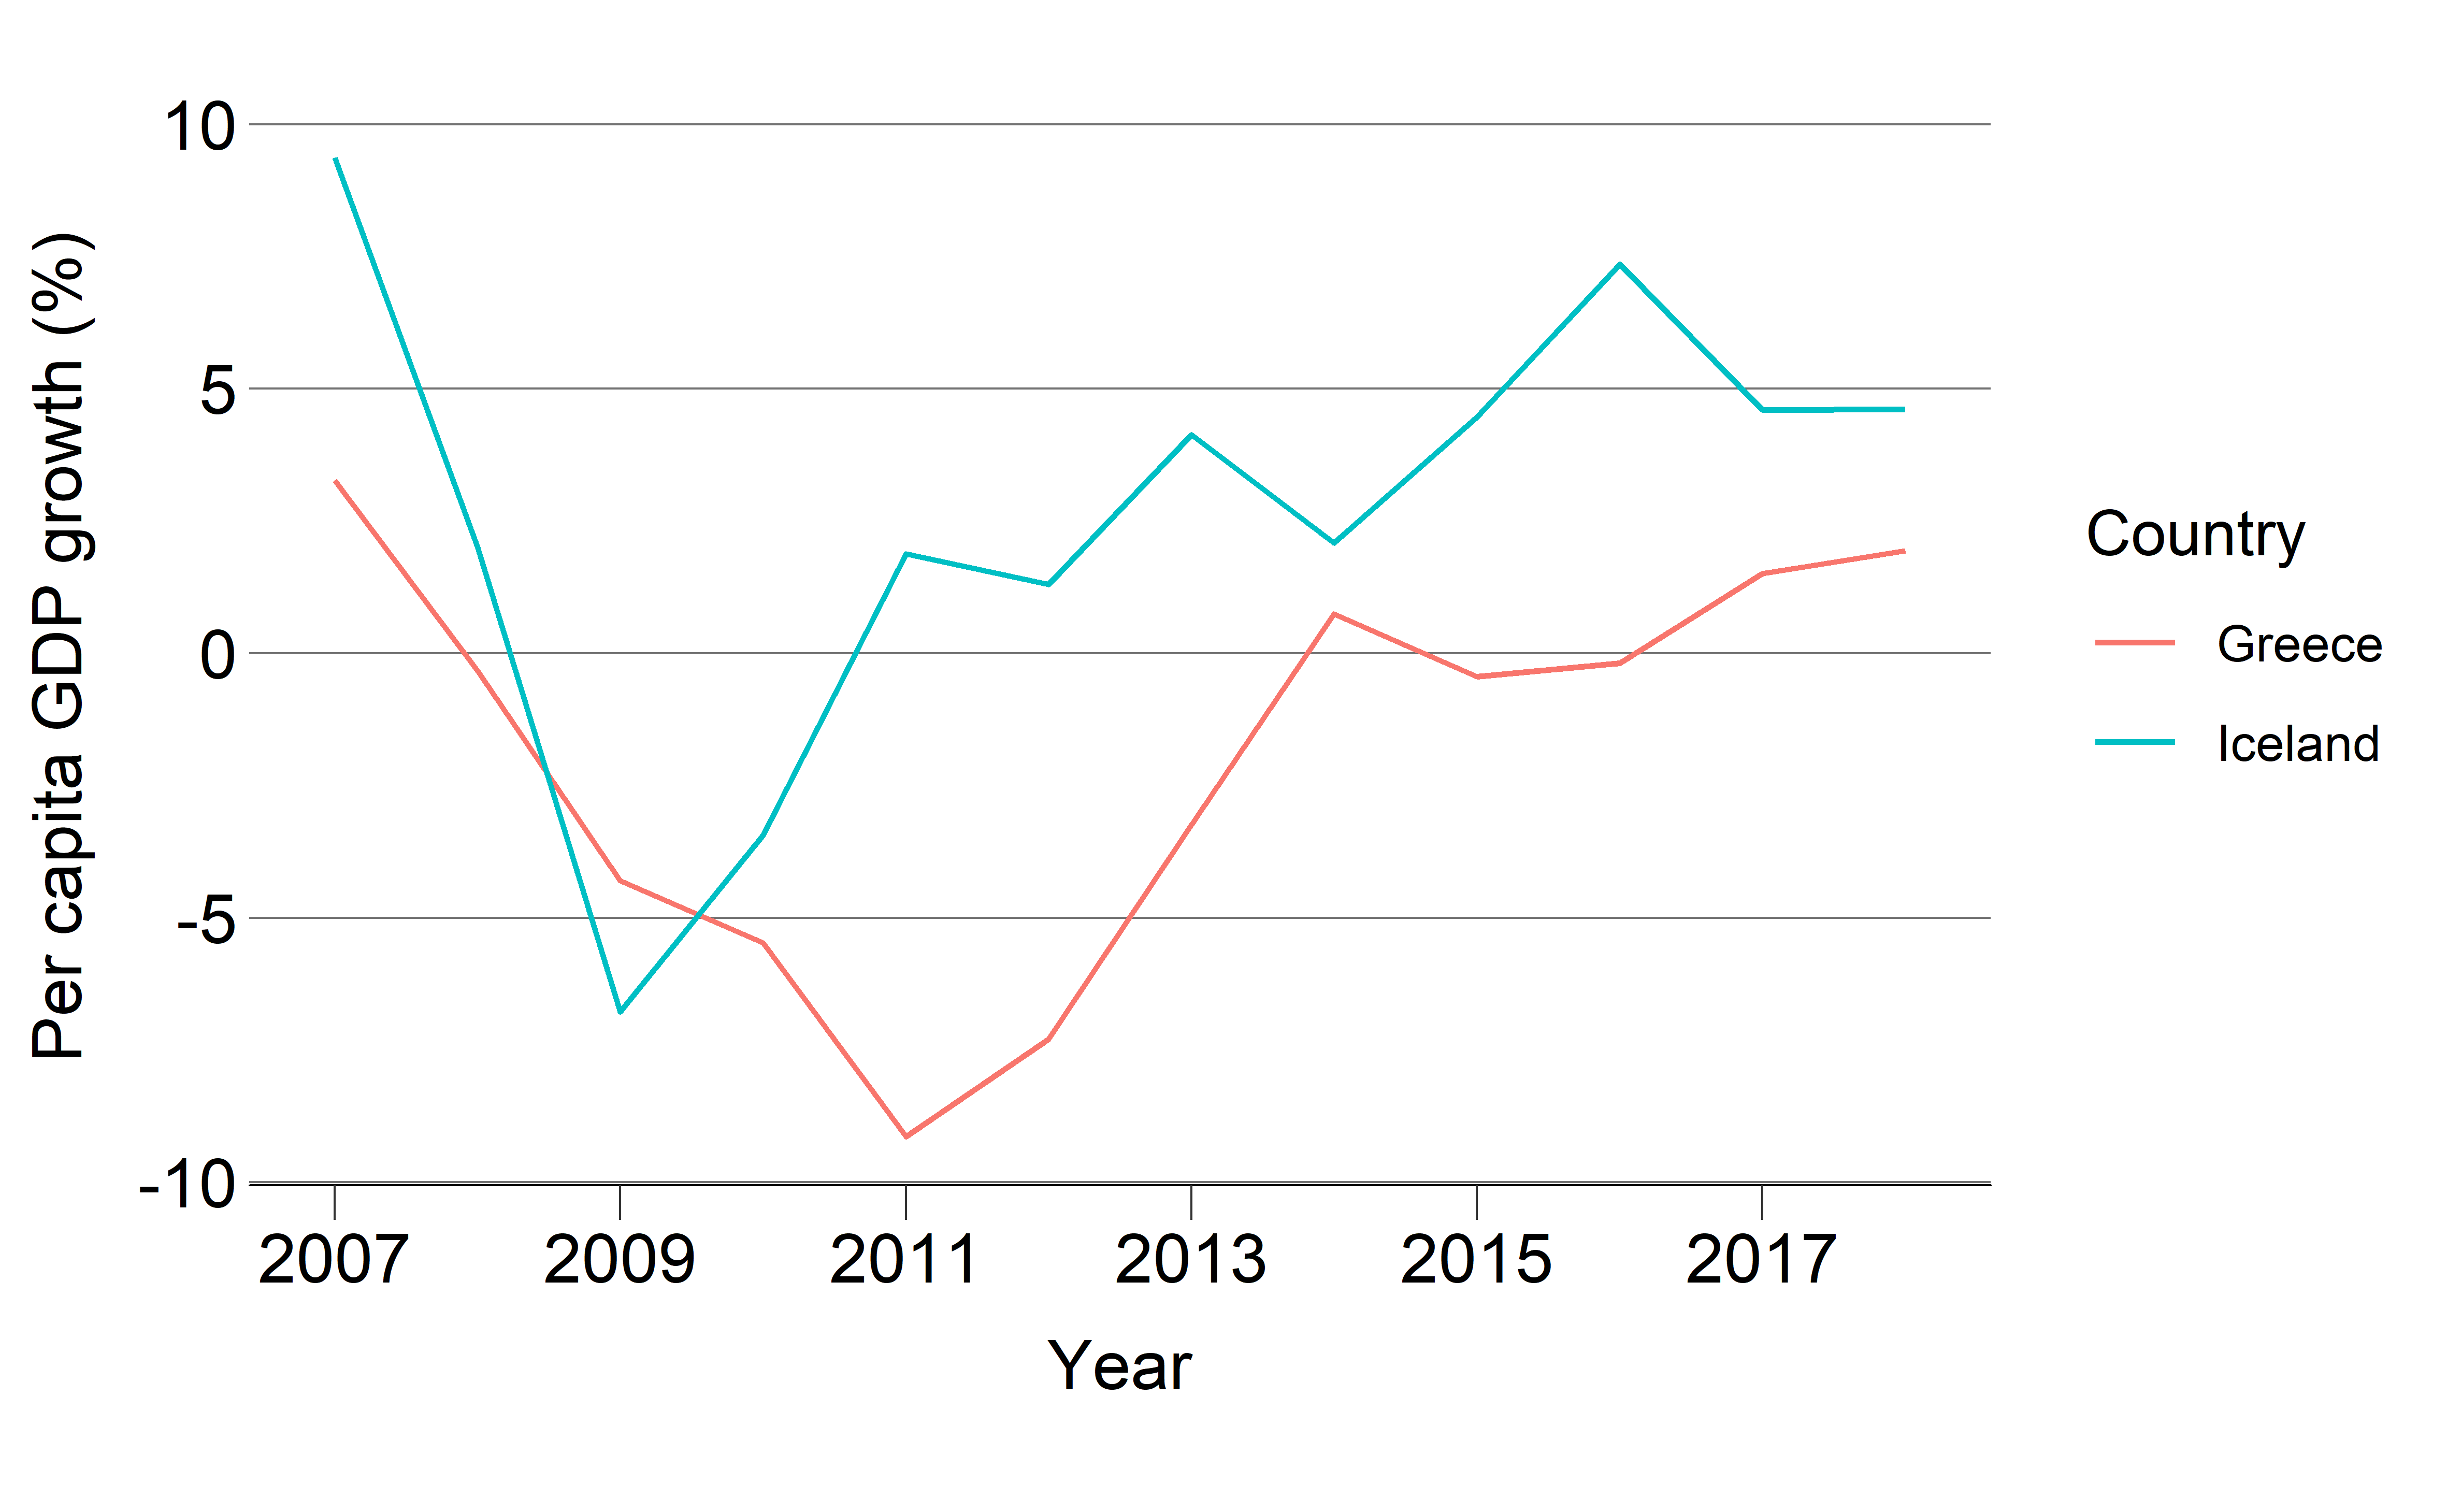
\includegraphics[width=\textwidth]{../img/greeceland.png}
\end{figure}{}
% Krugman might have a point!
% But, did Iceland really escape austerity? Imports did not catch up to pre-crisis levels until 2017. Selvsufficient in anluminium and fish...
\end{frame}{}

\begin{frame}{Lenders of last resort}
\begin{itemize}
    \item IMF, World Bank, ECB (Germany)\pause
    \item If not these then who?\pause % EU economy or already high inflation
    \item Moral hazard % Ferguson
\end{itemize}{}    
\end{frame}

\begin{frame}{}
\centering
\alert{\Large{Is the west going the way of Japan?}}
\begin{itemize}
    \item No/low growth, little/no inflation, low/negative interest rates
\end{itemize}{}
\end{frame}

% Youtube video if time

\end{document}
